\documentclass[a4paper,12pt]{report}
\usepackage{graphicx}
\pagestyle{myheadings}
\graphicspath { {'/'} }
\begin{document}
\author{Quang-Vinh Dang\\
COAST team - Inria}
\title{Technical Report\\ Performance measurement of collaborative editing tools}\maketitle

\section{Introduction}
Collaborative editing tools is an expanding filed in both research and application fields. There are many collaborative editing tools available at the moment, which allows multiple users collaborate on a single document at the same time from distance\footnote{An incomplete list of available tools can be found at: http://en.wikipedia.org/wiki/Collaborative\_real-time\_editor\#List\_of\_current\_editors}.

In this report, we want to evaluate the performance in term of delay between users, to see the adaptability of these tools in large scale settings.

The delay is defined as: the time since an user (the sender) did a modification on his local document (by using web browser) to the time since other users (the receivers) receive the modification on his local document.
There are two parameters are using to control the measurement:
	\begin{itemize}
		\item The number of users who modify a document at the same time\footnote{Google claimed that Google Docs can support up to 50 users to modify at the same time. Visit https://support.google.com/drive/answer/2494827?hl=en for more details}.
		\item The typing speed of users, in term of how many character has been send from keyboard of user per second\footnote{The average typing speed in composition is about 20 word per minute, or around 2 characters per second. The information at http://en.wikipedia.org/wiki/Typing}.
	\end{itemize}
\section{Measurement settings}
In this report, we perform the evaluation on three collaborative editing tools:
	\begin{description}
		\item [Google Docs\footnote{http://docs.google.com}] \hfill \\
			Google Docs is probably the most common collaborative editing tool, which provide an similar environment with Microsoft Office 2003 in your web browser.
		\item [Etherpad\footnote{http://etherpad.org/}] \hfill \\
			An open - source project with a very fast development speed
		\item [MUTE\footnote{http://mute-editorcrdt.rhcloud.com/}] \hfill \\
			A collaborative editing tool developed by COAST team, Inria Nancy, France.
	\end{description}
For using Etherpad and MUTE, we deployed both of them on the same server with the configuration: Intel Xeon W3550 (3.7GHz x 8), 8GB RAM, Ubuntu Server 14.04.1 LTS 64 bit\footnote{http://www.ubuntu.com/}.
The clients which run test used Ubuntu 14.10 64 bits.

The measurement is executed by using the following libraries and tools:
	\begin{itemize}
		\item Selenium\footnote{http://www.seleniumhq.org/}.
		\item xdotool\footnote{http://www.semicomplete.com/projects/xdotool/}.
	\end{itemize}
The result is processed by using:
	\begin{itemize}
		\item Python 2.7.+\footnote{https://www.python.org/}.
		\item R 3.1.2\footnote{http://www.r-project.org/}.
	\end{itemize}	 
To remove the difference in clock, the writing and reading users are simulated on a same computer. Other computers are used to simulate dummy writers.
\section{Result}
\subsection{Google Docs}
The result of the Google Docs experiment is as Fig. \ref{fig:fig1}. \textit{u} means number of users, and \textit{s} means typing speed in term of how many character were typed per second.

	\begin{figure}
		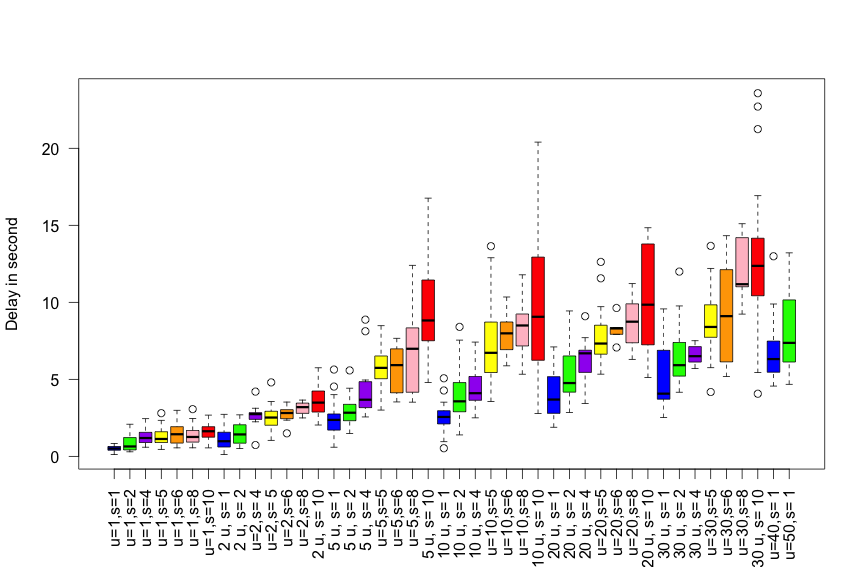
\includegraphics[width=\textwidth]{Rplot02}	
		\caption{Delays of Google Docs with different number of users and typing speed}
		\label{fig:fig1}
	\end{figure}
	
\subsection{Etherpad}
It seems that Etherpad is still in development phase. After the number of concurrent users exceed 20, Etherpad start to malfunction, such as show in Fig. \ref{fig:fig2} and Fig. \ref{fig:fig3}

	\begin{figure}
		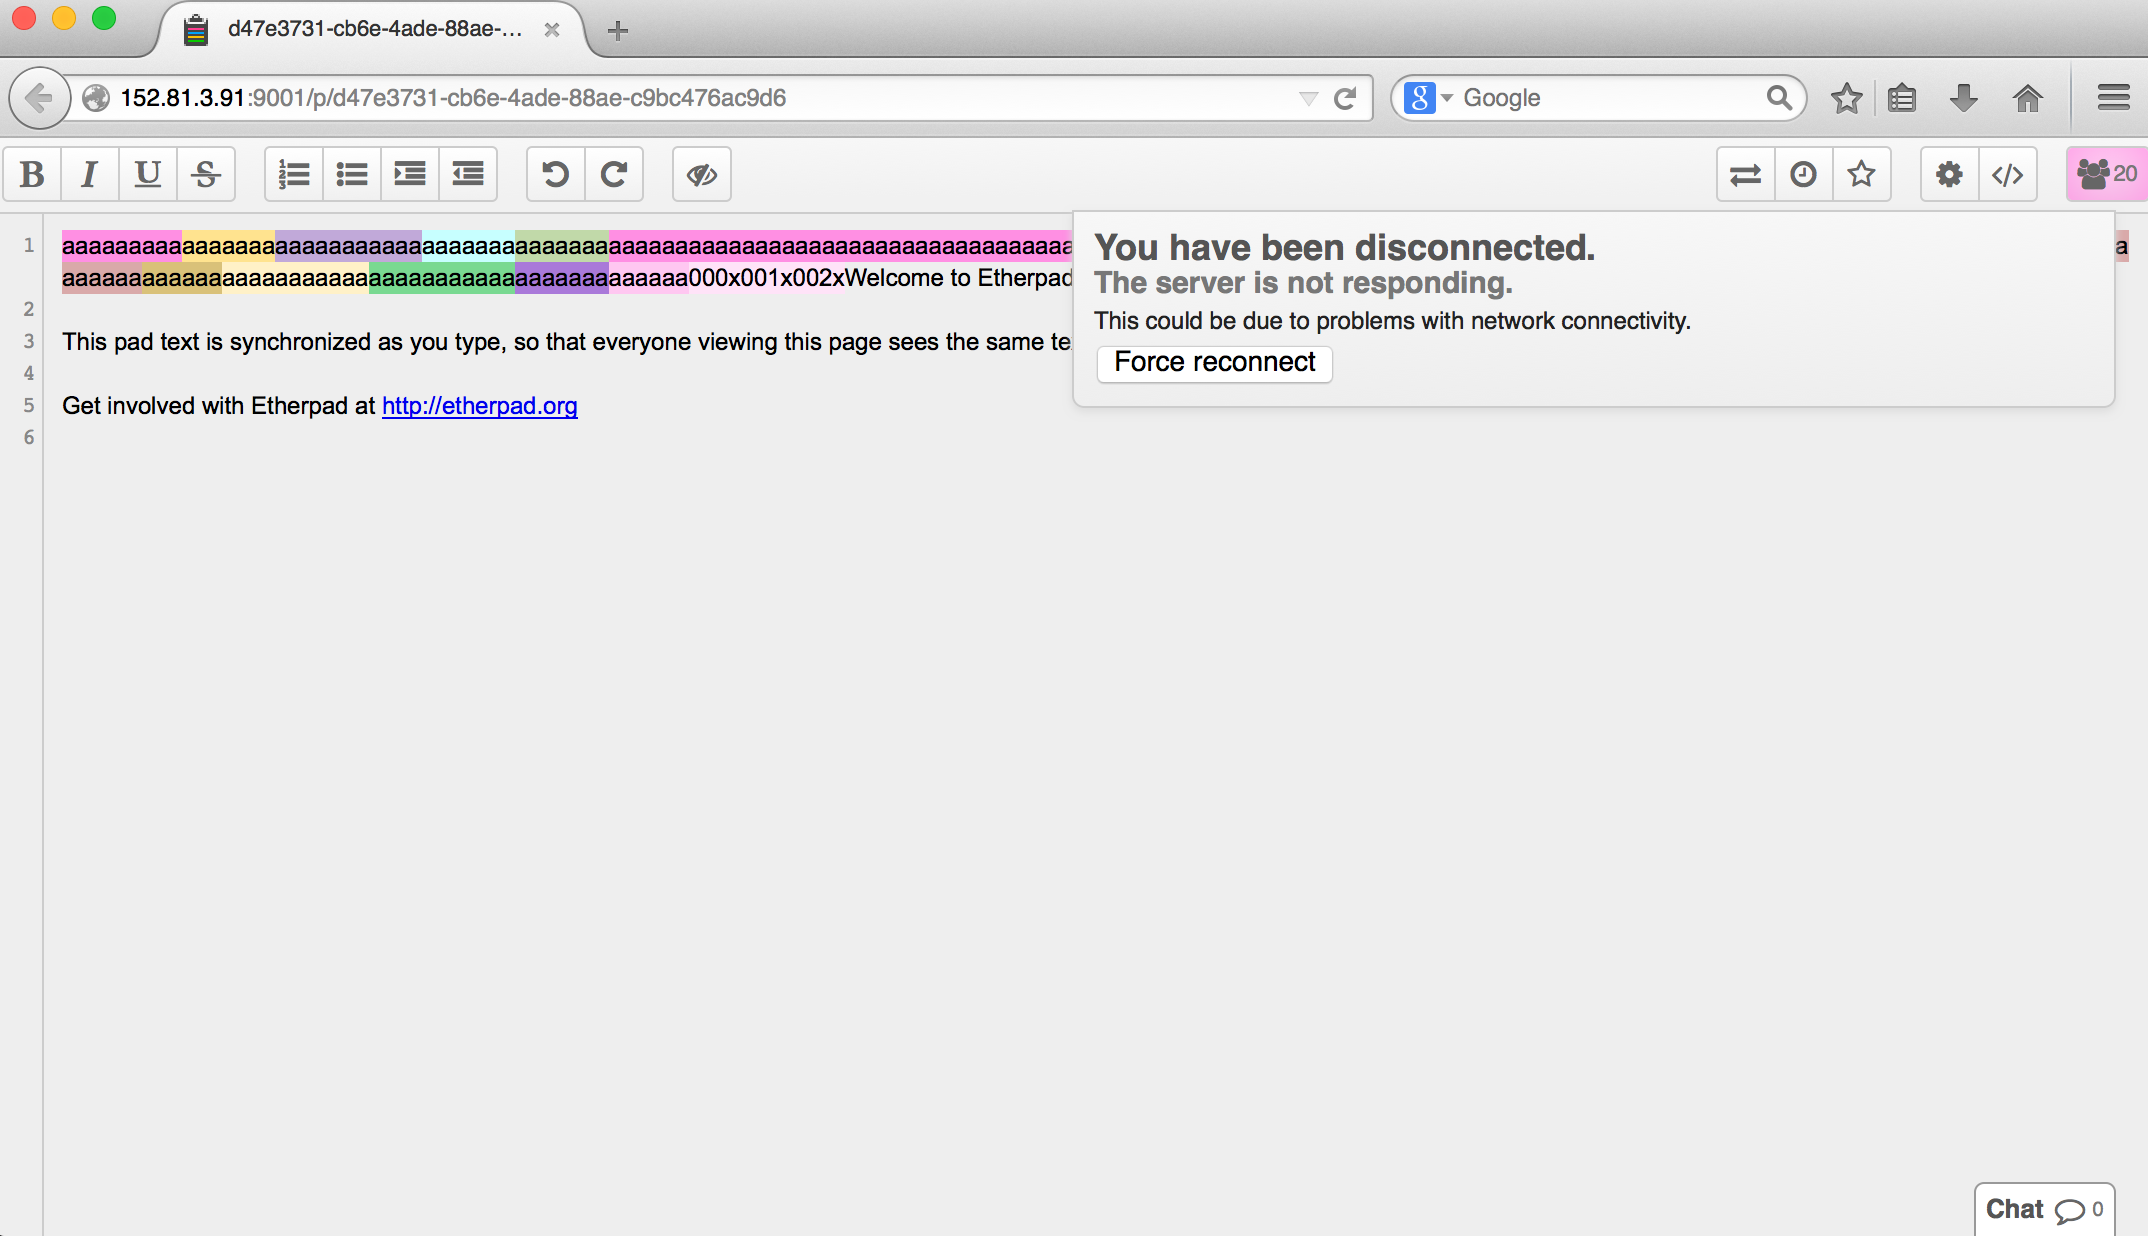
\includegraphics[width=\textwidth]{etherpad1}
		\caption{Etherpad server rejected clients after the number of clients reach to 20}
		\label{fig:fig2}
	\end{figure}

	\begin{figure}
		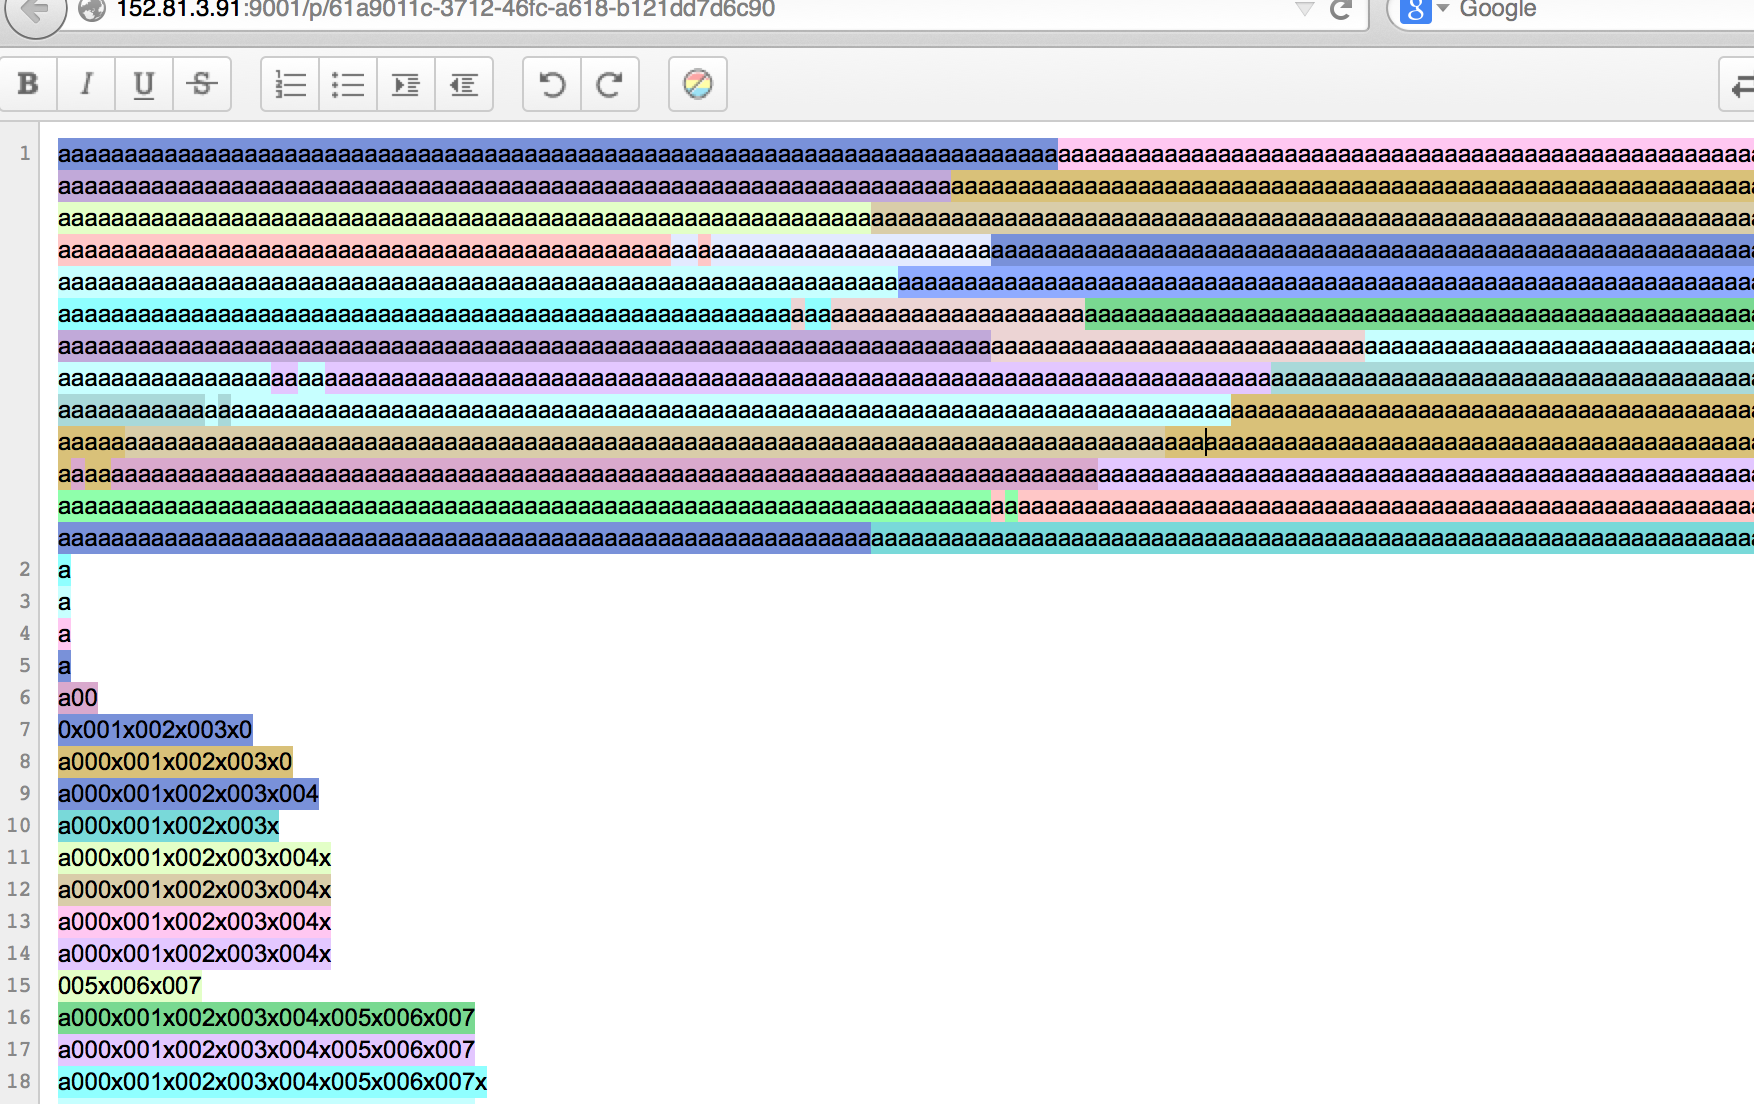
\includegraphics[width=\textwidth]{etherpad2}
		\caption{Etherpad start to be mess with a huge amount of request: the text 001x should appear only once}
		\label{fig:fig3}
	\end{figure}

\subsection{MUTE}
MUTE works quite well with the small number of users, and the most important point is the delay does not depend on the typing speed or number of user in a certain range.
The evaluation result of MUTE has been showed at Fig. \ref{fig:fig4}

	\begin{figure}
		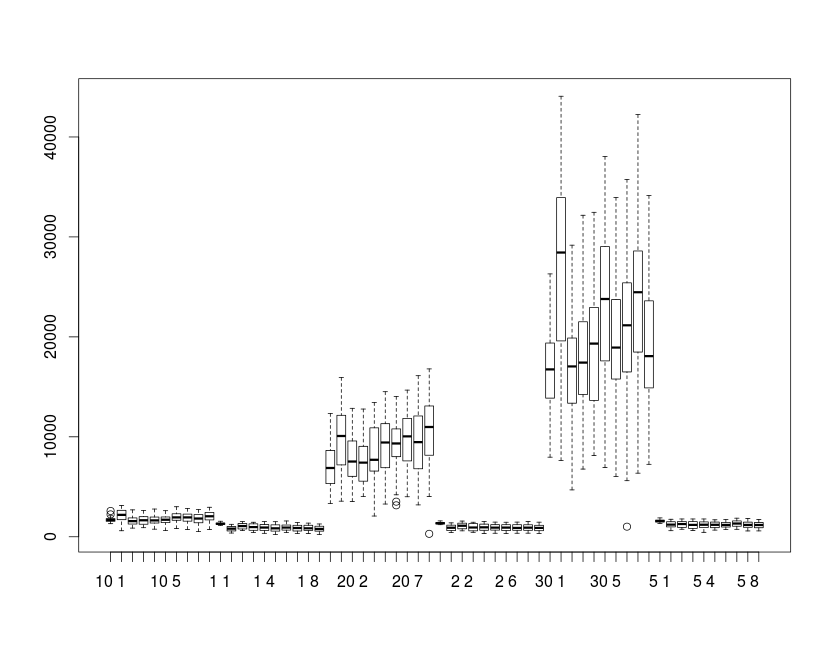
\includegraphics[width=\textwidth]{mute}
		\caption{Evaluation result of MUTE}
		\label{fig:fig4}
	\end{figure}
\section{Conclusion}
Google Docs is quite good for a small number of user with a slow typing speed (< 5 users and the typing speed is < 20 word per minute), but it does not work well with a large scale of user. We need some optimization and improvement to make the collaborative editing tool be suitable for a large scale of usage.

Etherpad needs to be improved more. Currently, it is only a proof of concept.

MUTE works very well until the server reach to its threshold. MUTE proved that it can be scale for a huge usage setting.

So far, there is no collaborative tools can deal with thousands of user or more, which we define as large scale collaboration.
\end{document}